\chapter{既存のシミュレータによる表現} \label{background}

本章では、斜方投射の例を通して既存のシミュレータである PhET~\cite{perkins_phet_2006} の表現方法ついて説明する。

\section{斜方投射}
斜方投射は、次のような現象である。
\begin{quote}
ある物体を原点から時刻 $t=0$ に、$x$ 軸方向の初速 $v_{0x}$ 、$y$ 軸方向の初速 $v_{0y}$ で投げる。このとき、重力加速度の大きさを $g$ とすると、物体は次のような軌道を描く。
$$
\left\{
\begin{aligned}
  x &= v_{0x} t \\
  y &= v_{0y} t - \dfrac{1}{2}gt^2 \\
\end{aligned}
\right.
$$
\end{quote}

\begin{figure}[H]
\centering
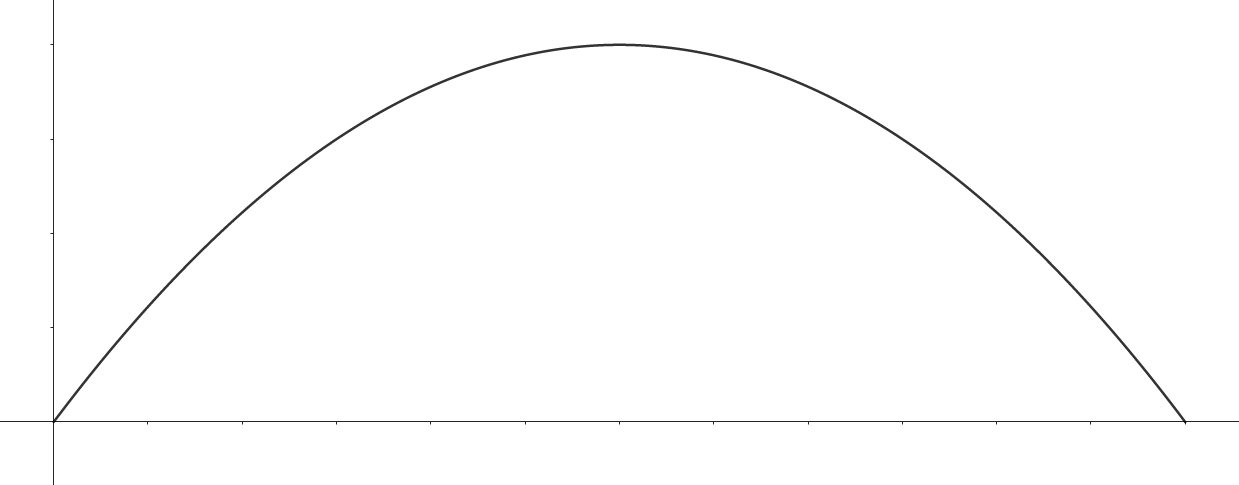
\includegraphics[width=0.9\linewidth]{figure/curve.png}
\end{figure}

\section{PhET による斜方投射の表現}

PhET (Physics Education Technology) は、コロラド大学ボルダー校によるプロジェクトで、物理学の教育に活用できるシミュレーションの作成を目標としている。2023年2月現在、ウェブサイト\footnote{\url{https://phet.colorado.edu}}上では50以上のシミュレーションが公開されている。また、物理学のみならず化学・数学・生物学・地球科学などのシミュレーションも公開されている。PhET を用いることで、実際の実験を行うのと同様な教育効果が得られる~\cite{ajredini_real_2014}(\ref{ajredini})。

図~\ref{numeral_based}は、PhET 上で斜方投射のシミュレーションを行った様子である。大砲から砲弾が射出されるという設定で表現されている。学習者は、初速度や砲弾の質量、仰角などを数値で指定することができ、着弾点を測定することができる。一方で、この軌道や着弾点の位置がどのように計算されたものなのかはわからない。


% 本章では、既存のシミュレータである PhET~\cite{perkins_phet_2006} を通して、現在のシミュレータでは不可能なことについて紹介し、\simname を用いることで解決できることを示す。

% PhET (Physics Education Technology) は、コロラド大学ボルダー校によるプロジェクトで、物理学の教育に活用できるシミュレーションの作成を目標としている。2023年2月現在、ウェブサイト\footnote{\url{https://phet.colorado.edu}}上では50以上のシミュレーションが公開されている。また、物理学のみならず化学・数学・生物学・地球科学などのシミュレーションも公開されている。PhET を用いることで、実際の実験を行うのと同様な教育効果が得られる~\cite{ajredini_real_2014}(\ref{ajredini})。

% PhET には様々なシチュエーションのシミュレータが存在するが、計測した値をどのように導出したかはわからない。例えば、図\ref{numeral_based} は放物運動を表現している。この軌道は、時刻を $t$ 、物体の $x$ 軸方向の初速を $v_{0x}$ 、$y$ 軸方向の初速を $v_{0y}$ として、
% \begin{align*}
%   x &= v_{0x} t \\
%   y &= v_{0y} t - \dfrac{1}{2}gt^2 \\
% \end{align*}
% と表される。しかし、シミュレータで計測した値がこのような方程式に基づいて計算されたということを直接確認することはできない。そのため、学習者はシミュレータで計測した数値が方程式と一致するかを計算によって確認するか、方程式で表現される運動を別の方法で描画し、シミュレータが描いた軌道に一致しているかを確認する必要がある。

% \simname を用いることで、上記の点が解決できる。\simname では、方程式を立式することで物理系を定義する。そのため、位置や速度などの値がどのような方程式に基づいて計算されたかを確認できる。また、\simname には現実の運動を正しく表現した動作例が存在する。これと比較しながら学習者自身が物理系を定義することで、方程式で表現された物理法則が現実の運動に対応していることを確認できる。
